%======================================================================
\section{Introduction}\label{sec:intro}
%======================================================================

\subsection{Positive solutions of the explicit formula}

Weil's explicit formula \cite{Wei52} (in Guinand's form \cite{Gui48} for $\zeta$) is a linear identity between a measure on the zeros of $\zeta$
and a measure on the prime powers. For even test functions $F$ in a natural class $\Tc$ (Definition~\ref{def:testclass}), with
$\hF(\xi)=\int F(t)e^{-2\pi i\xi t}\dd t$, it reads
\begin{equation}\label{eq:intro-EF}
\Arch(F)=\sum_\rho F\Big(\frac{\rho-\frac12}i\Big)+\frac1\pi\sum_{n\ge2}\frac{\Lambda(n)}{\sqrt n}\,\hF\Big(\frac{\log n}{2\pi}\Big),
\end{equation}
where $\Arch(F)$ depends only on the archimedean data of $\zeta$: its Gamma factor and its pole at $s=1$. Under the Riemann hypothesis (RH)
the right side is $\int F\dd\mu+\frac1\pi\int\hF\dd\nu$ for two positive measures, $\mu$ on the zero ordinates and $\nu$ on the points
$\xin n:=\log n/2\pi$. We ask how much of this structure is forced by positivity and the archimedean data alone. A \emph{positive solution}
of \eqref{eq:intro-EF}, or \emph{admissible pair} (Definition~\ref{def:admissible}), is a pair of positive measures, $\mu$ even on $\RR$ and
$\nu$ on $[\xin2,\infty)$, that represents $\Arch$ on $\Tc$; nothing else is assumed about their supports, and nothing about integrality.
Let $\Kad$ be the set of admissible pairs and $\pz$ the pair of $\zeta$, which is admissible exactly under RH.

\emph{Sharpness.} Testing \eqref{eq:intro-EF} against functions with $F\ge0$ and $\hF\ge0$ is the explicit-formula method of Stark, Odlyzko,
Poitou and Serre \cite{Sta74,Odl76,Ser75,Poi77,Odl90} for lower bounds on conductors and discriminants. For the archimedean data of $\zeta$ it
leads to the linear programme
\[
\kstar=\inf\Big\{\Arch(F):F\in\Cone,\ \int F=1\Big\},\qquad \Cone:=\{F\in\Tc:F\ge0\text{ on }\RR,\ \hF\ge0\text{ on }[\xin2,\infty)\},
\]
whose value $\kstar$ is the \emph{slack} of the data, and to its classical form, with value $\kOPS\ge\kstar$, in which $\Cone$ is replaced by
the cone $\ConeOPS$ of functions with $F\ge0$ and $\hF\ge0$ on all of $\RR$. A test function with $\Arch(F)=\kappa\int F$ proves the conductor
bound $e^{-2\pi\kappa}$, so $\qmin=e^{-2\pi\kstar}$ is the best bound the method can give (Part~I, Proposition~2.10). Is the method sharp for
$\zeta$ itself, that is, does it reach the conductor $1$ of $\zeta$? Odlyzko's numerical optimisation gave $0.997$ \cite[Table~4]{Odl90};
Part~I certified $\kstar\le1.4292\cdot10^{-1060}$, a conductor bound $1-8.98\cdot10^{-1060}$. By linear-programming duality, admissible pairs
exist if and only if $\kstar\ge0$ (Theorem~\ref{thm:I-duality}), a statement that involves neither zeros nor primes.

\emph{Uniqueness.} Do positivity and the archimedean data determine the solution, that is, is $\pz$ the only possible admissible pair?

Part~I \cite{Joh26} set up this framework and posed the two questions as Conjecture~S, $\kstar\le0$, and Conjecture~U, $\Kad\subseteq\{\pz\}$
(Section~\ref{sec:setting}). It proved Conjecture~U under support conditions, for instance when $\mu$ is carried by the zeros of $\zeta$ and
the origin (Theorem~\ref{thm:I-zerosupport}), and its magic-function principle (Corollary~\ref{cor:I-magic}) reduced Conjecture~U to the
construction of a function as in Theorem~\ref{thm:main-S} below whose real zeros are those of $\zeta$.

\subsection{Main results}

We answer both questions with an \emph{exact magic function}: an $F\in\Cone$ with $\int F>0$ and $\Arch(F)=0$
(Definition~\ref{def:magic}), which certifies $\kstar\le0$. The term comes from the linear-programming bounds for sphere packing of Cohn and
Elkies and of Viazovska \cite{CE03,Via17}, where such functions show that a bound is sharp.

Our function has the form $F=\Xi^2H$, with $\Xi(t)=\xi(\frac12+it)$ and $\xi(s)=\frac12s(s-1)\pi^{-s/2}\Gamma(\frac s2)\zeta(s)$. There is no
circularity in building $F$ from $\zeta$ itself: $\Xi$ vanishes at every non-trivial zero of $\zeta$, on or off the critical line, so the
factor $\Xi^2$ removes the zero side of \eqref{eq:intro-EF} without any information about where the zeros lie, and RH is assumed nowhere. The
explicit formula enters only as an unconditional identity, which turns $\Arch(F)$ into a sum over prime powers. The difficulty is to keep $F$
and $\hF$ non-negative; by Section~\ref{sec:reduction} this is a problem about the Gamma function and the integers alone.

\begin{mainthm}\label{thm:main-S}
There is an even entire function $H$, real on $\RR$, with $H(t)>0$ for every real $t$ and $H(0)=1$, such that for every $\delta\in(0,1)$
\begin{equation}\label{eq:intro-C1}
|H(z)|\le C_\delta\,(1+|z|)^{-9+\delta}\,e^{\pi|\Re z|/2}\qquad(|\Im z|\le\tfrac12+\delta),
\end{equation}
and such that $F:=\Xi^2H$ satisfies:
\begin{enumerate}[label=\textup{(\alph*)}]
\item $F\in\ConeOPS$: $F\ge0$ and $\hF\ge0$ on $\RR$;
\item $\hF(\xin n)=\hF'(\xin n)=0$ for every integer $n\ge2$;
\item $\int F=\hF(0)>0$ and $\Arch(F)=0$.
\end{enumerate}
Consequently $\kstar\le\kOPS\le0$. In particular Conjecture~S holds, and $\qmin\ge1$, already for the classical cone.
\end{mainthm}

Thus $F$ is an exact magic function, and the method of Odlyzko, Poitou and Serre is sharp for the data of $\zeta$, already in the classical
cone: $F$ proves the conductor bound $1$. Under RH no test function does better (Corollary~\ref{cor:main-RH}), so $F$ answers, in degree one,
Odlyzko's Open Problem~2.2 \cite[p.~123]{Odl90}: ``What functions $F(x)$ give the best GRH bounds for discriminants?'' We do not address the
unconditional Open Problem~2.1 of \cite{Odl90}, or higher degrees. Unconditionally, $F$ attains the least value $0$ of $\Arch/\!\int$ among the
cone members $\Xi^2H$ with $H$ analytic on a strip $|\Im t|\le\frac12+\delta$, all of which have $\Arch\ge0$ by Corollary~\ref{cor:I-zerokilling}.

\begin{mainthm}\label{thm:main-U}
Every admissible pair is $\zeta$'s pair: $\Kad\subseteq\{\pz\}$. That is, Conjecture~U holds.
\end{mainthm}

This is a rigidity statement: positivity and the archimedean data force any positive solution of \eqref{eq:intro-EF} to be carried by the zeros
of $\zeta$ and by the prime powers, with their usual weights. It follows from Theorem~\ref{thm:main-S} by complementary slackness: every
admissible pair is carried by the zeros of $F$ and of $\hF$ (Lemma~\ref{lem:I-compslack}), and, because $H>0$, the real zeros of $F$ are those
of $\zeta$, so the zero-side support theorem of Part~I (Theorem~\ref{thm:I-zerosupport}) applies.

\begin{maincor}\label{cor:main-RH}
The following are equivalent: \textup{(i)} RH; \textup{(ii)} admissible pairs exist; \textup{(iii)} $\kstar\ge0$; \textup{(iv)} $\kstar=0$. If they
hold, then $\Kad=\{\pz\}$, $\kOPS=0$, and $F/\int F$, with $F$ as in Theorem~\ref{thm:main-S}, is a minimiser for both $\kstar$ and $\kOPS$. If
RH fails, then $\kstar<0$ and $\Kad=\emptyset$.
\end{maincor}

\begin{remark}[The classical cone]\label{rem:intro-classical}
Part~I proves its duality theorem only at the gap $\xin2=\log2/2\pi$, where the prime powers begin. Corollary~\ref{cor:nogap} below removes
this restriction. The transform of the function $F$ of Theorem~\ref{thm:main-S} is positive on $(-\xin2,\xin2)$; so for every
$\ell\in[0,\xin2]$ a positive solution whose prime measure lives on $[\ell,\infty)$ puts no mass below $\xin2$, and a transfer lemma
(Lemma~\ref{lem:transfer}) carries the equivalences of Corollary~\ref{cor:main-RH} to the gap $\ell$. Appendix~\ref{app:gap} also proves the
duality theorem at every gap. For $\ell=0$, the classical cone, RH holds if and only if $\Arch\ge0$ on $\ConeOPS$, that is, if and only if
$\kOPS=0$. In the language of conductors: under RH the fully optimised explicit-formula bound for the data of $\zeta$ is exactly $1$ in either
cone, and if RH fails it exceeds $1$ in both. For gaps larger than $\xin2$ there are no positive solutions.
\end{remark}

The method does not prove too much: for the data of the Dedekind zeta functions of $\QQ(\sqrt5)$ and $\QQ(\sqrt{-3})$, Part~I certifies
strictly positive slack, so no exact magic function exists for them (Section~\ref{sec:remarks}).

\subsection{The explicit function}

The function $H$ of Theorem~\ref{thm:main-S} is explicit. Let $S(m,n;c)$ be the Kloosterman sum, $\Jdot:=\partial_\mu J_\mu|_{\mu=2}$,
$\Idot:=\partial_\mu I_\mu|_{\mu=2}$, and $\gi(t):=\frac12s(s-1)\pi^{-s/2}\Gamma(\frac s2)$ at $s=\frac12+it$, the archimedean factor of $\Xi$.

\begin{mainthm}[The object]\label{thm:main-object}
For $n\ge1$ put
\[
\Ss_n:=\sum_{c\ge1}\frac1c\Big[S(1,n;c)\,\Jdot\Big(\frac{4\pi\sqrt n}c\Big)-S(-1,n;c)\,\Idot\Big(\frac{4\pi\sqrt n}c\Big)\Big],\qquad
a_n:=n\Ss_n+\tfrac14\delta_{n1}.
\]
\begin{enumerate}[label=\textup{(\alph*)}]
\item The series converge absolutely, and with $z_n:=4\pi\sqrt n$ and $\abar_n:=n^{1/4}e^{4\pi\sqrt n}/(4\sqrt2\pi^2)$,
\[
\Big(1-\frac2{z_n}\Big)\abar_n\le a_n\le\abar_n\qquad(n\ge1);
\]
in particular every $a_n$ is positive.
\item The function $H$ of Theorem~\ref{thm:main-S} can be taken such that, for $x>1$,
\[
\int_\RR\gi(t)^2H(t)\,x^{-it}\dd t=C\,\sin^2(\pi x)\,\sqrt x\sum_{n\ge1}a_nK_0(4\pi\sqrt{nx}),\qquad C=880.6617\pm0.0015,
\]
and the left side equals $C/(32\pi^2)$ at $x=1$. Thus $b_n:=Ca_n$ satisfy
$(1-2/z_n)\cdot15.77370\,n^{1/4}e^{4\pi\sqrt n}\le b_n\le15.77376\,n^{1/4}e^{4\pi\sqrt n}$.
\item The left side of \textup{(b)} is, for every $x>0$, equal to $-C/(16\pi^2)$ times the four-path function \eqref{eq:GO}, which is analytic
on $\Re x>0$; and for real $t$, $H$ is given by the physical-side formula \eqref{eq:physical}: an integral of two $K_0$-series in the same
coefficients $a_n$ against $\cos(t\log Y)$ and against the positive conical kernel $\ck_t$.
\end{enumerate}
\end{mainthm}

The factor $\sin^2(\pi x)$ produces the double zeros at the integers; the sum $\sqrt x\sum_na_nK_0(4\pi\sqrt{nx})$ converges only for $x>1$, and
has a double pole at $x=1$, so the continuation to $(0,1]$ in (c) is part of the content.

Table~\ref{tab:coefficients} lists certified enclosures of the first coefficients and of $C$, for comparison with independent computations.
Figure~\ref{fig:object} illustrates $H$ on $[0,40]$ and the function in (b) on $[1,6]$; it is not part of any proof.

\begin{table}[b]
\centering
\small
\begin{tabular}{@{}lll@{}}
\toprule
 & certified ball & source\\
\midrule
$a_1$ & $4581.370553\pm0.000028$ & Kloosterman terms $c\le6\cdot10^5$, and a tail bound\\
$a_2$ & $1025727.23492\pm0.00011$ & Kloosterman terms $c\le6\cdot10^5$, and a tail bound\\
$a_3$ & $62590223.68999\pm0.00060$ & Kloosterman terms $c\le3\cdot10^5$, and a tail bound\\
$a_4$ & $1968035704.4549\pm0.0011$ & Kloosterman terms $c\le3\cdot10^5$, and a tail bound\\
$a_5$ & $40671323483.6182\pm0.0017$ & Kloosterman terms $c\le3\cdot10^5$, and a tail bound\\
$C$ & $880.6617\pm0.0015$ & Proposition~\ref{prop:C}\\
\bottomrule
\end{tabular}
\caption{The coefficients $a_1,\dots,a_5$ and the constant $C$ of Theorem~\ref{thm:main-object}, as certified balls
(Appendix~\ref{app:cert-coeffs} and Proposition~\ref{prop:C}). Each printed ball is rounded outward, so it contains the certified one.}
\label{tab:coefficients}
\end{table}

\begin{figure}[t]
\centering
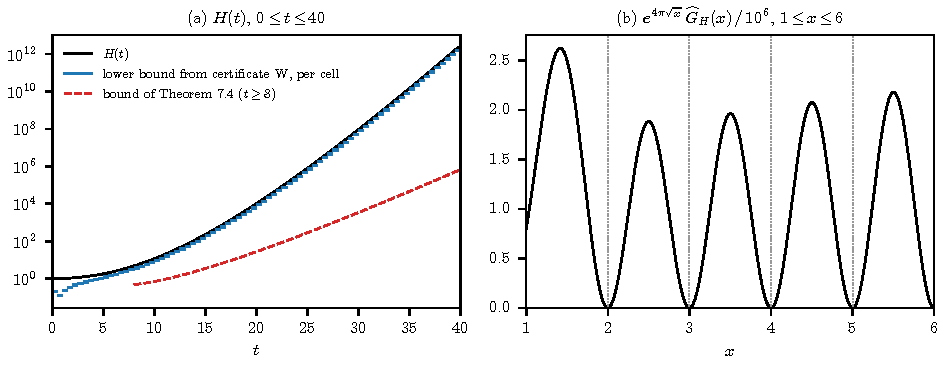
\includegraphics[width=\textwidth]{anc/figures/figure1.pdf}
\caption{An illustration; it is not part of any proof. (a) $H(t)$ for $0\le t\le40$, on a logarithmic scale. The curve joins $H(0)=1$ and the
values at the $80$ cell centres of the window certificate (Theorem~\ref{thm:window}), computed without error terms. The steps are lower
bounds for $H$ on each cell, formed from the certified cell bounds and the certified enclosure of $\Pi(0)$. The dashed curve is the bound of
Theorem~\ref{thm:large-t} for $t\ge8$. (b) $e^{4\pi\sqrt x}\,\Gh_H(x)/10^6$ for $1\le x\le6$, where $\Gh_H(x)$ is the left side of
Theorem~\ref{thm:main-object}(b), computed in floating point from the coefficient midpoints; $\Gh_H$ vanishes doubly at $x=2,\dots,6$, and
$\Gh_H(1)=C/(32\pi^2)$. Data and script: \ancf{figures/} in the ancillary files.}
\label{fig:object}
\end{figure}

\subsection{The construction in outline}

\emph{Reduction (Section~\ref{sec:reduction}).} For $F=\Xi^2H$ every zero of $\zeta$ is a zero of $F$, so $\Arch(F)$ is a sum over prime
powers (Corollary~\ref{cor:I-zerokilling}). On a line where the Dirichlet series of $\zeta^2$ converges absolutely, $\hF$ decouples, in the
variable $x$, into the positive combination $\sum_md(m)m^{-1/2}\,\Gh_H(mx)$ of dilates of the $\Gamma$-only transform
$\Gh_H(x)=\int\gi^2Hx^{-it}\dd t$ (Lemma~\ref{lem:voronoi}), so the integer zeros pass from $\Gh_H$ to $\hF$. So it suffices to find an even
$H$ of growth \eqref{eq:intro-C1} with $H\ge0$ whose $\Gamma$-only transform vanishes at every integer $x\ge2$ and is non-negative for
$x\ge2$: a \emph{$\Gamma$-only integer-critical function}. Arithmetic has disappeared from the problem; what remains is a question about the
Gamma factor and the lattice $\ZZ$.

\emph{Automorphic input (Section~\ref{sec:automorphic}).} The kernel $K_0(4\pi\sqrt{nx})$ arises by pairing the Whittaker function
$\sqrt vK_0(2\pi nv)$, of eigenvalue $\frac14$ for $\Delta=-v^2(\partial_u^2+\partial_v^2)$ on the upper half-plane, with the family
$\sqrt{xv}K_0(2\pi xv)$ (Lemma~\ref{lem:K0K0}), and $\sin^2(\pi x)$ is, up to the factor $-4$, the symbol of the second difference
$g(\tau+1)-2g(\tau)+g(\tau-1)$ acting on that family. So we look for a $1$-periodic eigenfunction of $\Delta$ with eigenvalue $\frac14$,
together with a partner whose second difference it is. We start from the odd Niebur--Poincar\'e series $P_\nu$ \cite{Nie73}, of eigenvalue $\frac14-\nu^2$,
whose Fourier coefficients are Kloosterman sums of $J_{2\nu}$ and $I_{2\nu}$ with an explicit constant (Theorem~\ref{thm:niebur-fourier}). The
first-order operator $2\partial_v+\nu^2/v$ maps eigenvalue $\frac14-\nu^2$ to $\frac14$ up to an error $(1-\nu^2)^2P_\nu/v$, which has a
\emph{double} zero at $\nu=1$ (Lemma~\ref{lem:jordan}); so the spectral derivative $\Pt=\partial_\nu[(2\partial_v+\nu^2/v)P_\nu]_{\nu=1}$ is an exact
eigenfunction with eigenvalue $\frac14$. It is $1$-periodic and odd, has no constant term, and decays exponentially at the cusp $\infty$, with
Fourier coefficients $-16\pi a_n$. It is not invariant under $\mathrm{SL}_2(\ZZ)$, so it is not a Maass cusp form; it is
the $Y^2$-component of a vector-valued function that is equivariant for the symmetric square of the standard representation, and its
$X^2$-component $\Phi=\Pt\circ S$ satisfies $\Phi(\tau+1)-2\Phi(\tau)+\Phi(\tau-1)=2\Pt(\tau)$.

\emph{Why eigenvalue $\frac14$, and why the symmetric square.} The eigenvalue $\frac14$ is that of $\zeta^2$: up to Gamma factors, $\zeta(s)^2$
is the $L$-function of the completed Eisenstein series at the centre $s=\frac12$, whose non-constant Fourier terms are multiples of
$d(|n|)\sqrt vK_0(2\pi|n|v)e(nu)$ (cf.~\cite{BC13}), and $d(m)$ is the weight in the decoupling of Section~\ref{sec:reduction}. Remark~\ref{rem:rep} explains heuristically why the symmetric square supplies the
first-order operator and the double root.

\emph{The lift (Section~\ref{sec:lift}).} We integrate the closed Green form $\omega(\Phi_j,k_\tau(x))$ of the weights $\Phi_j$ and of the kernel
$k_\tau(x)=\sqrt{xv}K_0(2\pi xv)\cos(2\pi ux)$ over four paths from the cusps to $i$, following the architecture of Viazovska's
construction (Section~\ref{ssec:related}); every weight vanishes on its own path. The result $\GO(x)$ is analytic for $\Re x>0$, equals $-16\pi^2\sin^2(\pi x)\sqrt x\sum
a_nK_0(4\pi\sqrt{nx})$ for $x>1$, and its Mellin transform, divided by the Gamma factor $\GR(w+\frac12)^2$, is even under $w\mapsto-w$ because the kernel intertwines $\tau\mapsto-1/\tau$ with
$w\mapsto-w$. The absence of constant terms in the cusp expansions makes $\GO$ vanish to order $x^{5/2}$ at $0$, and this makes $H$ entire. The
growth bound \eqref{eq:intro-C1} follows by integration by parts.

\emph{Positivity (Sections~\ref{sec:fourier} and~\ref{sec:physical}).} On the Fourier side, every $a_n$ is positive because the term $c=1$
dominates; the trivial bound $|S|\le c$ suffices for every $n$ (Theorem~\ref{thm:an-positive}). By the decoupling, the transform of
$\Xi^2H_{\rm raw}$ is then non-negative on $[0,\infty)$, hence on $\RR$ by evenness: $\Xi^2H_{\rm raw}$ is positive definite
(Proposition~\ref{prop:posdef}). So $\Xi(0)^2H_{\rm raw}(0)$, the integral of that transform, is positive, which fixes the sign of the normalisation
without computation; and $\Xi(t)^2H_{\rm raw}(t)$ is bounded below by an alternating polynomial in $t$ whose coefficients are moments of the
transform. A certified computation of sixteen moments gives $H>0$ for $|t|\le10.355$ (Theorem~\ref{thm:moments}). On the physical side, applying
the four-path functional to the Mellin transform of the kernel gives
\[
H_{\rm raw}(t)=\frac1{2\pi^2(t^2+\frac14)^2}\Big[\int_1^\infty\Ax(Y)\cos(t\log Y)\dd Y+\frac12\int_{1/2}^\infty\Bx(Y)\,\ck_t(\theta(Y))\dd Y\Big],
\]
where $\Ax,\Bx$ are $K_0$-series in the $a_n$ and the kernel $\ck_t$, built from conical Legendre functions, is positive by Mehler--Dirichlet's
formula (Theorems~\ref{thm:kernel-pos} and~\ref{thm:F}). An explicit lower bound for the kernel gives $H>0$ for $|t|\ge9$
(Theorem~\ref{thm:large-t-box}). Section~\ref{sec:assembly} assembles the proofs.

\subsection{What is computer-assisted, what is formalised, and what is not claimed}\label{ssec:claims}

\emph{Computer-assisted parts.} Exactly four ingredients rest on computations in rigorous ball arithmetic, each with a script and log in the
ancillary files (Appendix~\ref{app:cert}):
\begin{enumerate}[label=(\arabic*),leftmargin=*]
\item the moment certificate: $H>0$ for $|t|\le10.355$ (Theorem~\ref{thm:moments}), from sixteen moments;
\item the numerical inputs of the large-$|t|$ theorem (Proposition~\ref{prop:L-numbers-box}): the sign of $\Bx$ on $[0.90,4]$, one tail constant
$\bar\rho(4)<1$, and three integrals evaluated at $t=9$;
\item the certified enclosures of the coefficients $a_n$, from the Kloosterman terms with $c$ up to $6\cdot10^5$ and a tail bound from the Weil
bound, used in the proofs only for (4);
\item the value of the normalising constant $C$ (Proposition~\ref{prop:C}), which enters only Theorem~\ref{thm:main-object}(b) and
Table~\ref{tab:coefficients}.
\end{enumerate}
Items (1) and (2) use the coefficients only through the trivial-bound box of Section~\ref{sec:fourier}: the term $c=1$ of each $a_n$, and
$|S(\pm1,n;c)|\le\varphi(c)$ for the others. Everything else is proved analytically, including the positivity of every $a_n$ and the two-sided
bounds (their constants are elementary evaluations at the single point $z=4\pi$), the sign of $C$, and Corollary~\ref{cor:nogap}. Further
certified computations are independent checks, not used in the proofs of the main results: positivity on $[0,40]$ from the physical-side formula
(Theorem~\ref{thm:window}); the large-$|t|$ theorem from $t=8$ with the coefficients of (3) (Theorem~\ref{thm:large-t}); and the moment
certificate with the coefficients of (3). The deduction of Theorems~\ref{thm:main-S}--\ref{thm:main-U} and
Corollaries~\ref{cor:main-RH} and~\ref{cor:nogap} from the inputs listed in Remarks~\ref{rem:inputs} and~\ref{rem:nogap} is also checked in
Lean~4 (Appendix~\ref{app:lean}). Corollary~\ref{cor:nogap} is formalised as \texttt{rh\_iff\_kappaOPS\_zero} (with \texttt{corollary8\_2},
\texttt{corollary8\_2\_b}, \texttt{FT\_window}; Lemma~\ref{lem:transfer} as \texttt{transfer}), except the zero set in (a) and clause (c)(iv).
The inputs themselves are not formalised.

\emph{Not claimed.} We do not prove RH, or the existence of an admissible pair, which is equivalent to it (Corollary~\ref{cor:main-RH}). We do
not know whether $\kstar$ is attained when RH fails (under RH it is, by Corollary~\ref{cor:main-RH}) or whether the integer-critical function
is unique, and we claim nothing about the convergence of the exact Hermite family of Part~I or of other interpolation schemes. No bound on $H$
off the strip $|\Im z|\le\frac12+\delta$ is used or claimed; Remark~\ref{rem:infinite-type} sketches its growth there (order one, not of
exponential type).

\subsection{Related work}\label{ssec:related}

\emph{Magic functions and contour integrals.} Viazovska's solution of the sphere packing problem in dimension $8$ \cite{Via17} and its
extensions \cite{CKMRV17,CKMRV22} construct extremal functions for the linear programming bounds of Cohn and Elkies \cite{CE03} as $\sin^2$ times
Laplace transforms of modular forms, through contour integrals; Cohn and Gon\c{c}alves \cite{CG19} gave a sign-uncertainty analogue, and
Feigenbaum, Grabner and Hardin \cite{FGH21} studied the Fourier eigenfunctions of this type with prescribed zeros. In those settings positivity
is either visible or certified by interval arithmetic; Lee \cite{Lee26} proves algebraically the positivity, on the imaginary axis, of a family of
quasimodular forms that gives sign-uncertainty eigenfunctions of this type. Sections~\ref{sec:automorphic}--\ref{sec:lift} follow the
architecture of Viazovska's construction \cite{Via17}: $\Pt$ and $\Phi$ play the role of the depth-$2$ quasimodular form $\varphi_0$ and its
$S$-transform, the four paths and (up to a common factor) their weights are hers, and Green's identity replaces Cauchy's theorem. There are
partial precedents for non-holomorphic input: the closed Green form and the deformation of paths between cusps of Lewis and Zagier
\cite{LZ01}, and the Maass--Poincar\'e series that Radchenko and Sun \cite{RS25} continue in the spectral parameter to build Fourier
interpolation bases. Exact extremal functionals with double zeros at the expected spectrum also occur outside modular forms, in the conformal
bootstrap: Maz\'a\v{c} \cite{Maz17} constructs them for the one-dimensional bootstrap, and Hartman, Maz\'a\v{c} and Rastelli \cite{HMR19} adapt
such functionals to the modular bootstrap, where they reproduce the magic functions of dimensions $8$ and $24$. Extremal problems of Fourier
analysis attached to the explicit formula, mostly over band-limited test functions, are studied by Carneiro and coauthors, for instance for gaps
between primes \cite{CMS19} and for the pair correlation of zeros \cite{CCLM17}.

\emph{Zero-killing test functions.} The Fourier interpolation basis of Bondarenko, Radchenko and Seip \cite{BRS} and the interpolation theorem
of Radchenko and Viazovska \cite{RV19} are the analytic input of Theorem~\ref{thm:I-zerosupport}. The functions of that basis vanish, with
multiplicity, at every non-trivial zero of $\zeta$, on or off the critical line \cite[Theorem~1.1]{BRS}, and \cite[\S4.4]{BRS} reads
\eqref{eq:intro-EF} as the expansion of $\Arch$ in this basis. Devices that remove the zeros of $\zeta$ also appear elsewhere: Connes and
Consani \cite{CC23} note that the map $\mathcal E(f)(x)=x^{1/2}\sum_{n\ge1}f(nx)$, on even Schwartz functions with $f(0)=\widehat f(0)=0$, takes
values in the radical of the Weil quadratic form, and Benjamin and Chang \cite{BeCh22} remove the contributions of the zeros from a crossing
equation of the modular bootstrap with functionals whose Mellin symbol carries the factor $\zeta(s)$. Shen \cite{She26}, in an unrefereed
preprint, sets out the dictionary between the Cohn--Elkies bound and Weil's positivity criterion and shows that no compactly supported test
function can play, for $\zeta$, the role of the Cohn--Elkies magic function; the function $F$ of Theorem~\ref{thm:main-S} is not compactly
supported.

\emph{Niebur--Poincar\'e series and spectral derivatives.} Niebur \cite{Nie73} and Fay \cite{Fay77} introduced and expanded the series we use; the
expansion with the constant $2$ is stated by Bringmann, Jorgenson and Smajlovi\'c \cite[\S2.4]{BJS25}, and we prove it from scratch
(Lemma~\ref{lem:weyl}). Spectral derivatives of Poincar\'e and Eisenstein series at degenerate points appear in the theory of polyharmonic and
sesquiharmonic Maass forms: Andersen, Lagarias and Rhoades \cite[Theorem~1.1]{ALR18} describe the scalar critical point $s=\frac12$, Bringmann,
Diamantis and Raum \cite{BDR13} and Matsusaka \cite{Mat20} differentiate Poincar\'e series at harmonic points, and Alfes, Burban and Raum
\cite{ABR25} combine symmetric powers with spectral derivatives, in the framework of Bernstein and Gelfand \cite{BG80}, at eigenvalue $0$.

\emph{Period functions and self-reciprocity.} Lewis and Zagier \cite{LZ01} also introduced the Ferrar-type kernels of
eigenvalue-$\frac14$ forms; Bettin and Conrey \cite{BC13} treat the period function of the Eisenstein
series at $s=\frac12$, whose Voronoi kernel is $4K_0-2\pi Y_0$. The self-reciprocity of our $\Gamma$-only function under the Koshliakov kernel,
equivalent to the evenness of $H$, is the classical Mellin mechanism of Koshliakov, Dixit and others \cite{Kos29,Dix12,DM15,BDRZ17,DRRZ16}.

\emph{What is new.} To our knowledge the following are new: the function of Theorem~\ref{thm:main-object} and its coefficients; the
double-root lift of a spectral derivative of a Niebur--Poincar\'e series to an exact eigenfunction of eigenvalue $\frac14$, with its
symmetric-square partner; Viazovska's contour lift run with Green's identity on this non-holomorphic input; the positivity of $H$; the resulting
exact magic function for the explicit formula; and the criterion of Corollary~\ref{cor:nogap}. The positivity of the $a_n$ follows from the
standard dominance of the term $c=1$. Each ingredient has the precedents listed above; our search covered the standard bibliographic databases.
Section~\ref{ssec:history} describes how the function was found.

\subsection{Organisation}

Section~\ref{sec:setting} recalls the setting and the results of Part~I that are used, with full statements. Section~\ref{sec:reduction} proves
the reduction, Section~\ref{sec:automorphic} constructs the automorphic input, Section~\ref{sec:lift} the lift, and Sections~\ref{sec:fourier}
and~\ref{sec:physical} prove positivity. Section~\ref{sec:assembly} proves the main results, and Section~\ref{sec:remarks} discusses other
archimedean data, how the function was found, and open questions. Appendix~\ref{app:cert} describes the certificates, Appendix~\ref{app:bessel}
gives the Bessel-function bounds, and Appendix~\ref{app:gap} proves the transfer lemma used in Corollary~\ref{cor:nogap} and the duality
theorem at an arbitrary prime-side gap. Section~\ref{ssec:notation} collects the notation; in particular $x=e^{2\pi\xi}$ throughout, and
$\tau=u+iv$ is the variable on $\HH$.
